\section{Задача №1}

\subsection{Формулировка задачи}

\indent

О распределении температур в конечном стержне $x \in [0; l]$ с начальным распределением $T_{0} = 300 (a^{2} = 10^{-6})$ и источником тепла $f(x, t) = 300 (1 + e^{-t})$, когда на левом конце задана температура $\mu_{1}=500$, а правый - теплоизолирован. Исследовать ортогональность и нормировку собственных функций, построить графики $u(x, t)$, $l=0,1$ м.

\subsection{Постановка задачи}

\begin{numcases}{}
u_{t} = a^{2}u_{xx} + 300(1 + e^{-t}), \qquad\quad \!\text{$x\in(0;l); t > 0$;}\\
u(x, 0) = \varphi (x) = 300k = T_{0}, \qquad \text{$x\in(0;l); t = 0$;}\\
\left.
\begin{split}
u(0, t) &= \mu_{1},\qquad\qquad\qquad\qquad\quad \!\!\!\text{$x = 0; t > 0$;}\\
u_{x}(l, t) &= 0,\qquad\qquad\qquad\qquad\quad \text{$x = l; t > 0$}\\
\end{split}
\,\,\,\,\,\right]
\end{numcases}

\subsection{Теоретические сведения}

\indent

Рассмотрим часть стержня на отрезке $[ x, x + \Delta x ]$ и воспользуемся законом сохранения количества тепла, согласно которому общее количество тепла на отрезке $[ x, x + \Delta x ]$ равно сумме полного количества тепла, прошедшему через границы, и полного количества тепла, образованного внутренними источниками. Формула общего количества тепла, которое необходимо сообщить участку стержня, чтобы повысить его температуру на $\Delta u$: $\Delta Q = C \rho S \Delta x \Delta u$, где $C$ -- удельная теплоёмкость материала, $S$ -- площадь поперечного сечения. Формула количества тепла прошедшего через левый конец участка стержня за время $\Delta t$: $Q_{1} = -kSu_{x}(x, t)\Delta t$, где $k$ -- коэффициент теплопроводности материала.

Аналогично, тепловой поток через правый конец участка вычисляется по формуле: $Q_{2} = -kSu_{x}(x+\Delta x, t)\Delta t$.

По закону сохранения тепла:

$$\Delta Q = Q_{1} - Q_{2} \Rightarrow C\rho S\Delta x \Delta u = kSu_{x}(x+\Delta x, t)\Delta t - kSu_{x}(x, t)\Delta t$$

Поделим на $S\Delta x \Delta t$ и устремим $\Delta x$ и $\Delta t$ к нулю, получим:

$$\frac{C\rho S\Delta x \Delta u}{S\Delta x \Delta t} = \frac{kSu_{x}(x+\Delta x, t)\Delta t - kSu_{x}(x, t)\Delta t}{S\Delta x \Delta t} \Rightarrow C\rho u_{t}=ku_{xx},$$

\noindent так как $\frac{\Delta u}{\Delta t} \rightarrow u_{t}$, $\frac{u_{x}(x+\Delta x, t) - u_{x}(x, t)}{\Delta x} \rightarrow u_{xx}$,

\noindent тогда уравнение теплопроводности имеет вид: $u_{t}=a^{2}u_{xx}$, где $a=\sqrt{\frac{k}{C\rho}}$ - коэффициент температуропроводимости.

Если внутри стержня имеются непрерывно распределённые источники тепла, уравнение становится неоднородным и обретает вид: $u_{t} = a^{2}u_{xx}+f(x,t)$, где $f(x, t)=\frac{1}{C\rho S}q(x, t)$. 

\subsection{Решение задачи}

\indent

Представим решение в виде суммы: $u(x, t) = v(x, t) + \mu_{1}$. Будем приводить начально-краевую задачу (1)-(3) к задаче с однородными граничными условиями (3).

Представим $u(x, t)$ в таком виде в уравнение (1), получим:

$$v_{t} =  a^{2}v_{xx} + 300(1 + e^{-t}), \eqno (4)$$

в начальное условие (2):

$$
\begin{cases}
u(x, 0) = \left.(v + \mu_{1})\right|_{t=0} = v(x, 0) + \mu_{1} = T_{0}; \\
v(x, 0) = T_{0} - \mu_{1}
\end{cases}
\eqno (5)
$$

и в граничные условия (3):

$$
\begin{cases}
u(0, t) = \left.(v + \mu_{1})\right|_{x=0} = v(0, t) + \mu_{1} = \mu_{1}; \\
u_{x}(l, t) = \left.(v + \mu_{1})_{x}\right|_{x=l} = v_{x}(l, t) = 0; \\
v(0, t) = 0; \\
v_{x}(l, t) = 0
\end{cases}
\eqno (6)
$$

Найдём собственные функции задачи (4)-(6), но с однородным волновым уравнением:

$$v_{t} = a^{2}v_{xx} \eqno (7)$$

Метод Фурье разделения переменных:

$$ v(x, t) = X(x) \cdot T(t) $$

Подставим в (7):

$$X(x) \cdot T'(t) = a^{2}X''(x) \cdot T(t)$$

$$\frac{T'(t)}{a^{2}T(t)} = \frac{X''(x)}{X(x)} = -\lambda^{2} = const$$

Получим две обыкновенные дифференциальные линейные уравнения:

$$T'(t) + a^{2}\lambda T(t) = 0,$$
$$X''(x) + \lambda X(x) = 0.$$

Подставляя $v(x, t)$ в виде $X(x) \cdot T(t)$ в граничные условия (6), получим:

$$u(0, t) = X(0) \cdot T(t) = 0;\,\,\,u_{x}(l, t) = X'(l) \cdot T(t) = 0$$

Поскольку равенства должны выполняться тождественно (зная, что $T(t) \neq 0$), то:

$$X(0) = 0;\,\,\,X'(l) = 0$$

Получим задачу Штурма-Лиувилля:

$$
\begin{cases}
X''(x) - \lambda^{2}X(x) = 0; \\
X(0) = 0; \\
X'(l) = 0
\end{cases}
$$

Рассмотрим различные значения $\lambda^{2}$:

\makeatletter
\@fleqntrue
\makeatother

\begin{equation*}
  \begin{split}
    1)\,\,\lambda^{2} > 0:
  \end{split}
\quad\quad
  \begin{split}
    \begin{cases}
      X(x) & = C_{1}e^{-\lambda x} + C_{2}e^{\lambda x}; \\
      X(0) & = C_{1} + C_{2} = 0; \\
      X'(l) & = -\lambda C_{1}e^{-\lambda l} + \lambda C_{2}e^{\lambda l} = 0
    \end{cases}
  \end{split}
\end{equation*}

\begin{multline*}
\begin{vmatrix}
     C_{1} & C_{2}\\ 
     -\lambda C_{1}e^{-\lambda l} & \lambda C_{2}e^{\lambda l}\\
\end{vmatrix}
\neq 0 \Rightarrow \text{единственное решение, а} \Rightarrow  \\
\Rightarrow C_{1} = C_{2} = 0\text{, что не удовлетворяет условиям задачи.} 
\end{multline*}


\begin{equation*}
  \begin{split}
    2)\,\,\lambda^{2} = 0:
  \end{split}
\quad\quad
  \begin{split}
    \begin{cases}
      X(x) & = C_{1}x + C_{2}; \\
      X(0) & = C_{2} = 0; \\
      X'(l) & = C_{1} = 0
    \end{cases}
  \end{split}
\quad\Rightarrow\quad
C_{1} = C_{2} = 0\text{, что снова не удовл. условиям задачи.}
\end{equation*}

\begin{equation*}
  \begin{split}
    3)\,\,\lambda^{2} < 0:
  \end{split}
\quad\quad
  \begin{split}
    \begin{cases}
      X(x) & = C_{1}\sin{\lambda x} + C_{2}\cos{\lambda x}; \\
      X(0) & = C_{2} = 0; \\
      X'(l) & = \lambda C_{1}\cos{\lambda l} = 0
    \end{cases}
  \end{split}
\quad\quad\quad
l=\frac{(1 + 2n)\pi}{2}, n=0,1,2\ldots
\end{equation*}

\makeatletter
\@fleqnfalse
\makeatother

\begin{equation*}
  \begin{split}
    \boxed{\lambda_{n} = \frac{(2n + 1)\pi}{2l}}
  \end{split}
\quad\quad
  \begin{split}
    \boxed{X_{n} = \sin{\lambda_{n}x} = \sin{\frac{(1 + 2n)\pi}{2l}x}}
  \end{split}
\quad\quad
\end{equation*}

Проверим ортогональность собственных функций:

$$ ( X_{n}(x), X_{k}(x) ) = \int\limits_0^l \sin \left( \frac{\pi(1 + 2n)}{2l}x \right) \cdot \sin \left( \frac{\pi(1 + 2k)}{2l}x \right)dx = $$

$$ = \frac{1}{2}\int\limits_0^l \left( \cos \left( \frac{\pi(1 + 2n)x}{2l} - \frac{\pi(1 + 2k)x}{2l} \right) - \cos \left( \frac{\pi(1 + 2n)x}{2l} + \frac{\pi(1 + 2k)x}{2l} \right) \right)dx = $$

$$ = \frac{1}{2}\int\limits_0^l \left( \cos \left( \frac{\pi(n - k)x}{l} \right) - \cos \left( \frac{\pi(n + k)x}{l} \right)\right)dx\,\, \circled{=}$$

Если $n\neq k$, то:

$$\circled{=} \,\,\,\frac{1}{2} \left( \left. \frac{l}{\pi (n - k)} \sin \left( \frac{\pi (n - k)x}{l} \right) \right|_0^l - \frac{l}{\pi (n + k)} \sin \left( \left. \frac{\pi (n + k) x}{l} \right) \right|_0^l \right)=$$

$$ = \frac{1}{2} \left( \frac{l}{\pi (n - k)} \sin{(\pi (n - k))} - \frac{l}{\pi (n + k)} \sin{(\pi (n + k))} \right) = 0;$$

Если $n=k$, то:

$$\circled{=} \,\,\,\frac{1}{2}\int\limits_0^l \left( 1 - \cos \left( \frac{\pi(n + k)x}{l} \right) \right)dx = \frac{1}{2} \left( \left. x \right|_0^l - \cancelto{0}{\left. \frac{l}{\pi (n + k)} \sin \left( \frac{\pi (n + k)x}{l} \right) \right|_0^l} \right) = \frac{l}{2} $$

Квадрат нормы собственных функций:

$$\|X_{n}\|^{2} = \int\limits_0^l X_{n}^{2}(x)dx = \int\limits_0^l \sin^{2}{\lambda_{n}x}dx = \int\limits_0^l \frac{1 - \cos{2\lambda_{n}x}}{2}dx = \frac{l}{2} - \left. \frac{1}{4} \sin{2\lambda_{n}x}\right|_0^l = \frac{l}{2} $$

Решение задачи (4)-(6) с неоднородным уравнением будем искать в виде ряда по собственным функциям однородной задачи:

$$v(x, t) = \sum_{n=0}^{\infty}T_{n}(t)X_{n}(x) = \sum_{n=0}^{\infty}T_{n}(t)\sin \left( \frac{\pi (1 + 2n)}{2l}x \right)$$

Подставим функцию $v(x, t)$ в таком виде в неоднородное уравнение (4) в начальное условие (5):

$$\sum_{n=0}^{\infty}T'_{n}(t)\cdot \sin \left( \frac{\pi (1 + 2n)}{2l}x \right) = a^{2}\sum_{n=0}^{\infty} \left( -\frac{\pi^{2}(1 + 2n)^{2}}{4l^{2}} \right) T_{n}(t)\cdot \sin \left( \frac{\pi(1 + 2n)}{2l}x \right) + 300(1 + e^{-t}),$$

$$v(x, 0) = \sum_{n=0}^{\infty}T_{n}(0) \cdot \sin \left( \frac{\pi (1 + 2n)}{2l}x \right) = T_{0} - \mu_{1}.$$

Разложим неоднородность $300(1+e^{-t})$ в ряд Фурье по собственным \linebreak функциям $\left\{ \sin \left( \frac{\pi (1 + 2n)}{2l}x \right)  \right\}_{n=0}^{\infty}$.

$$300(1 + e^{-t}) = 300(1 + e^{-t}) \cdot \sum_{n=0}^{\infty} f_{n} \cdot \sin \left( \frac{\pi (1 + 2n)}{2l}x \right)$$

Коэффициенты разложения равны:

$$f_{n} = \frac{(1, X_{n}(x))}{\|X_{n}\|^{2}} = \frac{2}{l} \int\limits_0^l \sin \left( \frac{\pi(1 + 2n)}{2l}x \right)dx = \frac{2}{l} \cdot \left( - \frac{2l}{\pi (1 + 2n)} \right) \cdot \left. \cos \left( \frac{\pi(1 + 2n)}{2l}x \right) \right|_0^l=$$

$$ = - \frac{4}{\pi(1 + 2n)} \cdot \left( \cos \left( \frac{\pi(1 + 2n)}{2} \right) - 1 \right) = \frac{4}{\pi(1 + 2n)}$$

Подставляем полученное разложение в уравнение и начальное условие:

\begin{multline*}
\sum_{n=0}^{\infty}T'_{n}(t)\cdot \sin \left( \frac{\pi(1 + 2n)}{2l}x \right) = a^{2}\sum_{n=0}^{\infty} \left( -\frac{\pi^{2}(1 + 2n)^{2}}{4l^{2}} \right) \cdot T_{n}(t) \cdot \sin \left( \frac{\pi(1 + 2n)}{2l}x \right) + \\
+ 300(1 + e^{-t}) \cdot \sum_{n=0}^{\infty} f_{n} \cdot \sin \left( \frac{\pi(1 + 2n)}{2l}x \right),
\end{multline*}

$$\sum_{n=0}^{\infty}T_{n}(0) \cdot \sin \left( \frac{\pi(1 + 2n)}{2l}x \right) = (T_{0} - \mu_{1}) \cdot \sum_{n=0}^{\infty} f_{n} \cdot \sin \left( \frac{\pi(1 + 2n)}{2l}x \right),$$

Учитывая полноту системы собственных функций $\left\{ \sin \left( \frac{\pi (1 + 2n)}{2l}x \right)  \right\}_{n=0}^{\infty}$ на отрезке $[0; l]$ и сравнивая коэффициенты при одинаковых функциях $\sin \left( \frac{\pi (1 + 2n)}{2l}x \right)$, получим следующие задачи Коши для функций $T_{n}(t) (n=0,1,2\ldots).$

$$
\begin{cases}
T'_{n}(t) = - \frac{a^{2}\pi^{2}(1 + 2n)^{2}}{4l^{2}}T_{n}(t) + 300f_{n}(1 + e^{-t});\\
T_{n}(0) = (T_{0} - \mu_{1}) \cdot f_{n}
\end{cases}
$$

Общее решение уравнения:

$$T_{n}(t) = A_{n}e^{- \frac{a^{2}\pi^{2}(1 + 2n)^{2}}{4l^{2}}t} + T_{n_{\text{част}}}(t)$$

Частное решение неоднородного уравнения $T_{n_{\text{част}}}(t)$ ищем исходя из вида неоднородности, т.е. в виде:  

$$T_{n_{\text{част}}}(t) = C_{n} + D_{n}e^{-t}$$

Подставляем в уравнение:

$$-D_{n}e^{-t} = -\frac{a^{2}\pi^{2}(1 + 2n)^{2}}{4l^{2}}\left( C_{n} + D_{n}e^{-t}\right) + 300 f_{n} (1 + e^{-t})$$

\begin{equation*}
\begin{aligned}
e^{-t}: \\
\\
1:
\end{aligned}
\quad \left\{
\begin{aligned}
       -D_{n} & = -\frac{a^{2}\pi^{2}(1 + 2n)^{2}}{4l^{2}} D_{n} + 300f_{n} \\
       0 & = -\frac{a^{2}\pi^{2}(1 + 2n)^{2}}{4l^{2}} C_{n} + 300f_{n}
\end{aligned}
\right.
\end{equation*} 

Отсюда:

\begin{equation*}
  \begin{split}
    C_{n} = \frac{1200l^{2}f_{n}}{a^{2}\pi^{2}(1 + 2n)^{2}};
  \end{split}
\quad\quad
  \begin{split}
    D_{n} = \frac{300f_{n}}{\frac{a^{2}\pi^{2}(1 + 2n)^{2}}{4l^{2}} - 1} = \frac{1200l^{2}f_{n}}{a^{2}\pi^{2}(1 + 2n)^{2} - 4l^{2}};
  \end{split}
\end{equation*}

$$T_{n_{\text{част}}}(t) = \frac{1200l^{2}f_{n}}{a^{2}\pi^{2}(1 + 2n)^{2}} + \frac{1200l^{2}f_{n}}{a^{2}\pi^{2}(1 + 2n)^{2}-4l^{2}} \cdot e^{-t}=$$

$$= 1200l^{2}f_{n} \left( \frac{1}{a^{2}\pi^{2}(1 + 2n)^{2}} + \frac{e^{-t}}{a^{2}\pi^{2}(1 + 2n)^{2} - 4l^{2}} \right)$$

$$T_{n}(t) = A_{n}e^{-\frac{a^{2}\pi^{2}(1 + 2n)^{2}}{4l^{2}}t} + 1200l^{2}f_{n} \left( \frac{1}{a^{2}\pi^{2}(1 + 2n)^{2}} + \frac{e^{-t}}{a^{2}\pi^{2}(1 + 2n)^{2} - 4l^{2}} \right)$$

Коэффициенты $A_{n}$ найдём из начального условия:

$$T_{n}(0) = A_{n} + 1200l^{2}f_{n}  \left( \frac{1}{a^{2}\pi^{2}(1 + 2n)^{2}} + \frac{1}{a^{2}\pi^{2}(1 + 2n)^{2} - 4l^{2}} \right) = (T_{0} - \mu_{1})f_{n}$$

$$A_{n} = (T_{0} - \mu_{1})f_{n} - 1200l^{2}f_{n} \left( \frac{1}{a^{2}\pi^{2}(1 + 2n)^{2}} + \frac{1}{a^{2}\pi^{2}(1 + 2n)^{2} - 4l^{2}} \right)$$

\begin{multline*}
T_{n}(t) =  \left( (T_{0} - \mu_{1})f_{n} - 1200l^{2}f_{n} \left( \frac{1}{a^{2}\pi^{2}(1 + 2n)^{2}} + \frac{1}{a^{2}\pi^{2}(1 + 2n)^{2} - 4l^{2}} \right) \right)e^{-\frac{a^{2}\pi^{2}(1 + 2n)^{2}}{4l^{2}}} + \\
+1200l^{2}f_{n}\left( \frac{1}{a^{2}\pi^{2}(1 + 2n)^{2}} + \frac{e^{-t}}{a^{2}\pi^{2}(1 + 2n)^{2} - 4l^{2}} \right) = 
\end{multline*}

$$ = (T_{0} - \mu_{1})f_{n}e^{-\frac{a^{2}\pi^{2}(1 + 2n)^{2}}{4l^{2}}t} + 1200l^{2}f_{n}\left( \frac{1}{a^{2}\pi^{2}(1 + 2n)^{2}} + \frac{e^{-t}}{a^{2}\pi^{2}(1 + 2n)^{2} - 4l^{2}} \right) \cdot (1 - e^{-\frac{a^{2}\pi^{2}(1 + 2n)^{2}}{4l^{2}}t}).$$

$\Rightarrow$ решение задачи (4)-(6) имеет вид:

\begin{multline*}
v(x, t) = \sum_{n=0}^{\infty}f_{n} \left( (T_{0} - \mu_{1})e^{-\frac{a^{2}\pi^{2}(1 + 2n)^{2}}{4l^{2}}t} + 1200l^{2} \left( \frac{1}{a^{2}\pi^{2}(1 + 2n)^{2}} + \frac{e^{-t}}{a^{2}\pi^{2}(1 + 2n)^{2} - 4l^{2}} \right) \cdot \right. \\ 
\left. \cdot \left( 1 - e^{-\frac{a^{2}\pi^{2}(1 + 2n)^{2}}{4l^{2}}t} \right) \right) \cdot \sin {\frac{\pi(1 + 2n)}{2l}x}
\end{multline*}

Решение задачи (1)-(3) будет:

$$u(x, t) = \mu_{1} + \sum_{n=0}^{\infty}f_{n} \left( (T_{0} - \mu_{1})e^{-\frac{a^{2}\pi^{2}(1 + 2n)^{2}}{4l^{2}}t} + 1200l^{2} \left( \frac{1}{a^{2}\pi^{2}(1 + 2n)^{2}} + \frac{e^{-t}}{a^{2}\pi^{2}(1 + 2n)^{2} - 4l^{2}} \right) \cdot \right.$$

$$\left. \cdot \left( 1 - e^{-\frac{a^{2}\pi^{2}(1 + 2n)^{2}}{4l^{2}}t} \right) \right) \cdot \sin \left( {\frac{\pi(1 + 2n)}{2l}x} \right) = \mu_{1} + \sum_{n=0}^{\infty} \frac{4}{\pi(1 + 2n)} \left( (T_{0} - \mu_{1})e^{-\frac{a^{2}\pi^{2}(1 + 2n)^{2}}{4l^{2}}t} + \right. $$

$$ \left. + 1200l^{2} \left( \frac{1}{a^{2}\pi^{2}(1 + 2n)^{2}} + \frac{e^{-t}}{a^{2}\pi^{2}(1 + 2n)^{2} - 4l^{2}} \right) \cdot \left( 1 - e^{-\frac{a^{2}\pi^{2}(1 + 2n)^{2}}{4l^{2}}t} \right) \right) \cdot \sin \left( {\frac{\pi(1 + 2n)}{2l}x} \right)$$

Подставим $l = 0,1 \text{м}; a^{2} = 10^{-6}; \mu_{1} = 500; T_{0} = 300$:

\begin{multline*}
u(x, t) = 500 + \sum_{n=0}^{\infty} \frac{4}{\pi(1 + 2n)} \left( -200e^{\frac{-\pi^{2}(1 + 2n)^{2}}{4 \cdot 10^{4}}t} + 12 \left( \frac{10^{6}}{\pi^{2}(1 + 2n)^{2}} + \frac{10^{6}e^{-t}}{\pi^{2}(1 + 2n)^{2} - 4 \cdot 10^{4}} \right) \cdot \right. \\
\left. \cdot \left( 1 - e^{-\frac{\pi^{2}(1 + 2n)^{2}}{4 \cdot 10^{4}}t} \right)\right) \sin{(5\pi(1 + 2n)x)} \end{multline*}

\pagebreak

Построим графики функции $u(x, t)$ в разные моменты времени:

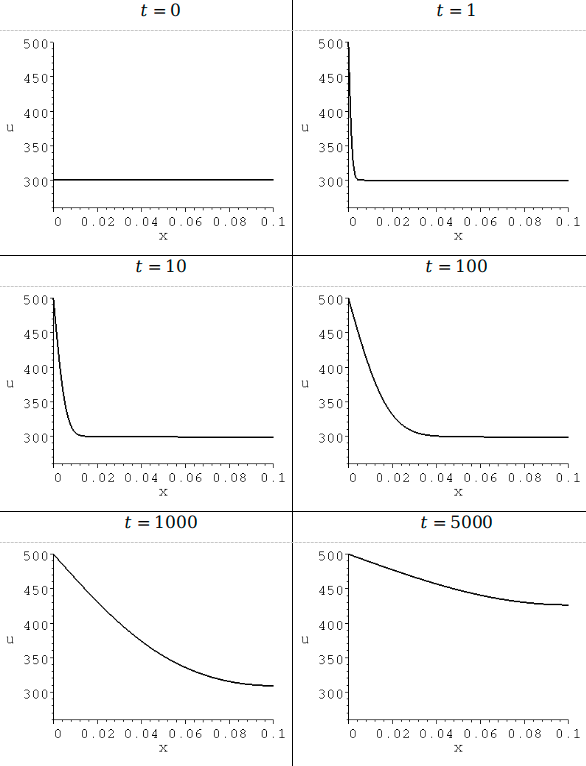
\includegraphics[width=0.8\linewidth]{task1.png}

По этой картине можно сказать следующее, при $t = 0$ значение $u$ будет равным 300, что верно, благодаря условию $u(x, 0) = \varphi(x)$. При изменении $t$ мы видим, что график функции $u(x, t)$ принимает своё начало в 500, что тоже верно, благодаря другому условию: $u(0, t) = \mu_{1}(t)$. При небольших $t$ можно чётко увидеть, как функция $u$ к концу стержня стремится к 300, что соответствует условию $u_{x}(l, t) = 0$. В целом график функции полностью соответствует краевым условиям задачи.

\pagebreak